\documentclass[12pt]{article}
\usepackage{anysize}
\marginsize{1.2cm}{1.4cm}{.4cm}{1cm}

\usepackage[normalem]{ulem}
\usepackage{amsfonts}
\usepackage{amsmath}
\usepackage[shortlabels]{enumitem}
\usepackage[font=small,labelfont=bf]{caption}
\usepackage{graphicx}
\usepackage{listings}
\usepackage{hyperref}
\usepackage{tikz}
\lstset{
  basicstyle=\ttfamily,
  mathescape
}

\setlength{\parindent}{0pt}

\title{Using Search to Synthesize a Distributed Program}
\date{Summer 2021}
\author{Ian Dardik}

\begin{document}

\maketitle

\section{Intro}
This note is the formal description of the program synthesis problem I am trying to solve as well as a proposal for implementation.  Here is a high level description of the problem: \\

A user wants to create a distributed program and already has a good idea of what their desired algorithm looks like.  However, the user does not want to write the algorithm by hand because they do not want to debug a distributed program.  Instead, the user can input a precise statement of requirements to the synthesizer to produce a program that is guaranteed to satisfy all the given requirements.  The more precise the given requirements are, the more likely we are to synthesize a program that the user desires.  The user can think of developing a requirement spec for the synthesizer as analogous to writing a program; they may need to go through an iterative process of testing and updating their requirement spec to achieve their desired program.  However, unlike writing a program in a programming language, users can guarantee their desired requirements will hold by construction.  


\section{Formal Problem Description}
\subsection{The Problem}
The inputs are:
	\begin{enumerate}
		\item State variables.  
		\item Initial state.  
		\item Required states.  
		\item Safety requirements.  Deadlocks are automatically considered a violation.  
		\item Liveness requirements.  
		\item The set of all possible instructions in the program.  
	\end{enumerate}

Given these inputs, the program will either output a program that satisfies the given requirements, an error, or will time out with no solution.  Search continues due to the following three reasons:
\begin{enumerate}
	\item There are still states left on the queue.  No states on the queue means that all possible programs have safety violations and we return an error.  
	\item There are still required states that haven't been visited.  
	\item There are still outstanding liveness requirements.  
\end{enumerate}

If we find a program that visits all required states and has no outstanding liveness requirements then we return success.  

\subsection{States}
The user will provide the name of each state variable as well as its domain.  Note that because the state variables are given, we can view our problem as a variant of a protocol completion problem.  We may have the user to mark variables with permissions (e.g. rwrw where the 1st two bits are permissions for other processes and the 2nd two bits are permissions for a process' own variables), but this may not be necessary due to the fact that the user supplies the instruction set.  

\subsection{Stationary States}
We will refer to ``Stationary States" throughout this document.  A Stationary State is a state in which all liveness requirements can be fulfilled.  Both the state and the instruction history determine whether all of a process' liveness requirements \textit{are} fulfilled; but a Stationary State only requires that a process' liveness requirements \textit{can} be fulfilled.  For example, imagine that a process has a single state variable ``on" and a single liveness requirement ``on $~\sim>$ ring bell" (ring bell is some output event).  Let the initial state be ``on $=False$".  The initial state is a Stationary State because all liveness requirements can be (and are) fullfilled.  Notice that if the process sets ``on $=True$" then ``on = $False$" and never rings the bell then the process will be in a Stationary State but will not have fulfilled all of its liveness requirements.  \\

Stationary States are important because they show an absense of a liveness requirement; any process in a stationary state cannot be trusted to make a move, and hence cannot be trusted to participate in helping to achieve a goal.  This is particularly important in Peterson's Algorithm; if we make the initial state stationary then we can avoid synthesizing a round-robin style algorithm because no process can be trusted to cooperate.  Instead, the synthesizer will be forced to find a solution where individual processes can enter the critical section without requiring the help of other processes.  

\subsection{Required States}
The user may specify a subset of states that the program must visit.  This may seem like a liveness requirement, but we do NOT consider it a liveness requirement here.  Instead, we see this as a guide to help the synthesizer produce an algorithm that the user desires.  In practice this means that we should not expect required states to be a motivator for processes to make progress.  This is imortant for an algorithm like Peterson's where the intial state needs to be stationary, but the algorithm we desire needs to eventually enter the critical section.  

\subsection{Input Language}
The safety and liveness requirements will be specified using an input language that will likely resemble TLA+.  The input language is very important because it defines the expressive power that the user has to describe a specific program; the richer the language, the more power a user has to specify a program that they want and will find useful.  The language will allow arbitrary safety requirements (in 1st order logic), but for the time being I will only allow a conjunction of ``leads to" ($~\sim>$) expressions for specifying liveness.  In this document I will talk about the input as described by the input language, however, in practice I will hard code all inputs to avoid dealing with parsers and ASTs (at least for the first cut).  

\subsection{Instruction Set}
The list of all possible instructions that the program can execute.  This replaces the previous idea of a ``transition constraint".  I will hard code a function for each instruction for the time being.  

\section{Examples}
\subsection{Peterson's}
We will describe a set of requirements that should synthesize an algorithm that is close to Peterson's Mutual Exclusion Algorithm.  Assume $ProcSet = \{0,1\}$, then:
	\begin{enumerate}
		\item State variables: cs (critical section): local, flag: global, turn: global.  Their type signatures are: \\
				$\forall p \in ProcSet : cs[p] \in \{TRUE,FALSE\}$ \\
				$\forall p \in ProcSet : flag[p] \in \{TRUE,FALSE\}$ \\
				$turn \in ProcSet$
		\item Initial state: $turn = 0$, $\forall p \in ProcSet: \lnot cs[p] \wedge \lnot flag[p]$
		\item Required state: $\forall p \in ProcSet : cs[p]$.  In other words, each process must be able to enter the critical section at some point.  
		\item Safety requirements:
			\begin{enumerate}
				\item $\forall p,q \in ProcSet : cs[p] \wedge cs[q] => p = q$ (mutual exclusion)
				\item $\forall p \in ProcSet : cs[p] => flag[p]$
			\end{enumerate}
		\item Liveness requirements:
			\begin{enumerate}
				\item $\forall p \in ProcSet : flag[p] ~\sim> cs[p]$
				\item $\forall p \in ProcSet : flag[p] ~\sim> \lnot flag[p]$
				\item $\forall p \in ProcSet : cs[p] ~\sim> \lnot cs[p]$
			\end{enumerate}
		\item Instruction Set: Approximately: flip $flag[p]$, flip $cs[p]$, flip $turn$, $turn = Other(p)$, $turn = p$, wait $turn[p]$, wait $flag[q]$, wait $turn[p] \wedge flag[q]$, wait $turn[p] \vee flag[q]$
	\end{enumerate}

Assuming the synthesizer produces a program without timing out, let's see what guarantees we can make for the following three properties \cite{mutex}:
	\begin{enumerate}
		\item Satisfies Mutual Exclusion: given by the safety property (a)
		\item Satisfies Progress: this is given by the safety property (a),  the state requirement, and the fact that the initial state is a Stationary State.  The fact that the initial state is stationary means that any process that enters the critical section cannot rely on any other process to help them; this prevents the synthesizer from producing a round-robin style algorithm.  Safety property (a) implies that any process that wants to enter the critical section must assume that all other processes \textit{may} also attempt to enter the critical section, and must cooperate with those processes to achieve its goal.  The state requirement guarantees that the synthesizer will not stop working until it finds an algorithm that enters the critical state.  
		\item Does not satisfy Bounded Waiting: we will synthesize a program that \textit{does} have a bounded amount of time for how long it takes a process to enter the critical section once it expresses intent; however, that time bound is arbitrary and is not guaranteed to limit the number of times other processes can enter the critical section.  
	\end{enumerate}

I may need to think more about how to express the Bounded Waiting requirement, but I don't necessarily see this as a must-do before implementation.  

\subsection{ABP}
We will describe a set of requirements that should synthesize an algorithm that is close to Alternating Bit Protocol.  Assume $ProcSet = \{0,1\}$ and the set $Data$ is given, then:
	\begin{enumerate}
		\item State variables: send, rec.  Their type signatures are: \\
				$\forall p \in ProcSet : send[p] \in Data \times \{0,1\}$ \\
				$\forall p \in ProcSet : rec[p] \in Data \times \{0,1\}$
		\item Initial state: $\exists d \in Data : \forall p \in ProcSet : send[p] = rec[p] = (d,0)$
		\item Required state: $\forall p \in ProcSet : send[p][2] = 1$.  In other words, the algorithm must advance to send at least one data item.  Note that sequences are 1-indexed like in TLA+.  
		\item Safety requirements:
			\begin{enumerate}
				\item $\forall p,q \in ProcSet : send[p][2] = rec[q][2] => send[p][1] = send[q][1]$
				\item $\forall p,q \in ProcSet : send[p][1] \neq rec[q][1] => send[p][2] \neq send[q][2]$
			\end{enumerate}
		\item Liveness requirements:
			\begin{enumerate}
				\item $\forall p,q \in ProcSet : send[p] \neq rec[q] ~\sim> send[p] = send[q]$
			\end{enumerate}
		\item Instruction Set: Approximately: $\exists p \in ProcSet : send[p][1] = rand(Data) \wedge send[p][2] = 1-send[p][2]$, $\exists p \in ProcSet : rec[p] = send[p]$
	\end{enumerate}


\section{Implementation}
Consider the following algorithm for synthesizing a program for $p$ processes using a BFS:
	\begin{verbatim}
		input: requirements
		queue = [noop]
		while true:
		  program = pop(queue)
		  for instruction in AllInstructions:  // branching exp
		    newProgram = program + instruction
		    if satisfiesAllRequirements(newProgram, requirements):  // interleaving exp
		      return newProgram
		    if noSafetyViolations(newProgram, requirements):  // interleaving exp
		      add(queue, newProgram)
	\end{verbatim}

Note that there are two nested exponentials here:
	\begin{enumerate}
		\item The branching factor that is $O(b^n)$, where $b=|AllInstructions|$ (the number of available instructions) and $n$ is the number of lines in the program
		\item The time it takes to check all interleavings of the $p$ processes to make sure that all requirements are satisfied in a given program.  
	\end{enumerate}

I believe these are the two nested exponentials mentioned in \cite{asdp}, however I may be wrong.  Either way, this is clearly very expensive.  Below I will talk about ideas for combating each exponential separately.  

\subsection{Efficiently Checking For Safety Violations}
\subsubsection{Probabilistic Analysis}
To guarantee that a program satisfies all safety properties we must check every possible interleaving of instructions for all $p$ processes.  With a bit of help from the internet \cite{il}, we find that the number of possible interlreavings of $n$ instructions with $p$ processes is $$f(n,p)=\frac{(pn)!}{(n!)^p}$$

Suppose we only want to check a single interleaving for a violation, let us calculate the probability of checking the correct one.  There exists a finite trace $\tau$ that contains the safety violation, with the last state being the perpetrator \cite{def}.  If the safety violation was introduced at instruction $i$, then at least one of the $f(i,p)$ interleavings contain $\tau$ as a prefix; let's call this $\tau_i$.  At instruction $j$ (where $j \geq i$) there are $f(j-i,p)$ interleavings that contain $\tau_i$ as a prefix.  This implies that the probability that a random interleaving with $j$ instructions finds the safety violation is: $$\frac{f(j-i,p)}{f(j,p)}$$

Suppose, for a program with $n$ instructions, we choose $g(n)$ interleavings independently and randomly to check for safety violations.  Then the probability we find the safety violation $\tau$ \textit{by the time} we have $j$ instructions is at least:
$$1 - \prod\limits_{k=i}^j \left(1 - \frac{f(k-i,p)}{f(k,p)}\right)^{g(k)}$$

Analytically, I was not able to figure out whether this probability is high or low.  It was simple enough to test the results with a program though, and I discovered that the probability of finding the safety violation by checking a polynomial number of interleavings (i.e. $g(n) = O(n^c)$, $c$ is a constant) is dismally bad as $i$, the instruction where a violation is introduced, increases.  This is not good news for the worst case scenario.  However, it may be the case that when safety violations are introduced, they appear in many of the interleavings.  Let us assume that the safety violation at instruction $i$ is introduced to $c$ percent (expressed as a decimal) of the interleavings; this means that there are $c*f(i,p)$ interleavings with a safety violation at instruction $i$.  This implies that the probability of finding a safety violation introduced at instruction $i$ by the time we reach instruction $j$ is:
$$1 - \prod\limits_{k=i}^j \left(1 - \frac{c*f(i,p)*f(k-i,p)}{f(k,p)}\right)^{g(k)}$$

I made a bit of progress here analytically but I want to double check my work before I include it.  

\subsubsection{Results and Discussion}
I tested this in a program where $j=i+1$, $p=2$, $c=1*10^{-6}$, and $g(n) = 1000 * n^2$ and the results are very promising:
\begin{verbatim}
	rand=1.00000, diff=1.00000 | f(i,p)=1.000000e+00, g(i,p)=1.000000e+00, i=0, j=1
	rand=0.58700, diff=0.80423 | f(i,p)=1.847560e+05, g(i,p)=1.000000e+05, i=10, j=11
	rand=0.46521, diff=0.49338 | f(i,p)=1.378465e+11, g(i,p)=4.000000e+05, i=20, j=21
	rand=0.75052, diff=0.77703 | f(i,p)=1.182646e+17, g(i,p)=9.000000e+05, i=30, j=31
	rand=0.91378, diff=0.96443 | f(i,p)=1.075072e+23, g(i,p)=1.600000e+06, i=40, j=41
	rand=0.97793, diff=1.00000 | f(i,p)=1.008913e+29, g(i,p)=2.500000e+06, i=50, j=51
\end{verbatim}

And again with $j=i+5$:
\begin{verbatim}
	rand=1.00000, diff=1.00000 | f(i,p)=1.000000e+00, g(i,p)=1.000000e+00, i=0, j=5
	rand=0.89315, diff=0.99838 | f(i,p)=1.847560e+05, g(i,p)=1.000000e+05, i=10, j=15
	rand=0.73746, diff=0.89312 | f(i,p)=1.378465e+11, g(i,p)=4.000000e+05, i=20, j=25
	rand=0.93940, diff=0.99230 | f(i,p)=1.182646e+17, g(i,p)=9.000000e+05, i=30, j=35
	rand=0.99186, diff=0.99999 | f(i,p)=1.075072e+23, g(i,p)=1.600000e+06, i=40, j=45
	rand=0.99936, diff=1.00000 | f(i,p)=1.008913e+29, g(i,p)=2.500000e+06, i=50, j=55
\end{verbatim}

Where:
\begin{itemize}
	\item ``rand" is the probability of finding a violation if we randomly check $g(i,p)$ interleavings, independently choosing a random interleaving each time (described above)
	\item ``diff" is the probability of finding a violation if we randomly check $g(i,p)$ interleavings, purposely choosing a different interleaving at each instruction level (not described above)
	\item ``f(i,p)" is the total number of interleavings at $i$ instructions and $p=2$ processors
	\item ``g(i,p)" is the number of interleavings we check
	\item ``i" is the instruction number at which the safety violation is introduced
	\item ``j" is the instruction number that we calculate the probability of finding the safety violation for
\end{itemize}

The number of possible interleavings increases exponentially ($1e29$ when $i=50,j=51$) while the number of interleavings we choose to check increases quadratically and remains far more managable ($2.5e6$ when $i=50,j=51$).  Furthermore, the probability of finding a safety violation converges towards 1 as $i$ increases.  \\

Assuming that safety violations are introduced in batches that are a fixed percentage of the number of interleavings is a big assumption.  However, if it is valid, it can drastically reduce the number of checks we need to perform while still yielding a high percent chance of catching safety violations after just a few rounds of adding instructions.  If the assumption is invalid the consequences are large: we pay an exponential price ($O(b^n)$) per branch that we \textit{could} have pruned if we correctly detected the safety violation.  Fortunately, missing safety violations only impacts performance; we can always do a full check of all interleavings for a program once it satisfies all requirements (I would likely need to use an SMT solver in practice) before returning it to the user as a correct solution.  \\

In short, this idea may be able to reduce the number of interleavings we need to check from factorial time down to polynomial time (quadratic in the example I checked).  


\subsection{Efficiently Searching For Programs}
\subsubsection{Liveness Graph Analysis}
All liveness properties are in the form of ``leads to" so we can create a directed graph where each node represents a subset of states, and each edge represents a ``leads to".  Taking Example 3.1 (Peterson's):

\begin{center}
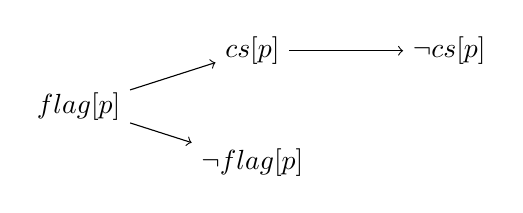
\begin{tikzpicture}[node distance={10mm}, main/.style = {}]
\node[main] (1) {$flag[p]$};
\node[main] (2) [above right of=1, xshift=15mm] {$cs[p]$};
\node[main] (3) [below right of=1, xshift=15mm] {$\lnot flag[p]$};
\node[main] (4) [right of=2, xshift=15mm] {$\lnot cs[p]$};
\draw[->] (1) -- (2);
\draw[->] (2) -- (4);
\draw[->] (1) -- (3);
\end{tikzpicture}
\end{center}

If there are multiple (unconnected) graphs then we can be sure they are separated by Stationary States.  It may be easier to reject any specifications whose liveness properties aren't connected to make the problem simpler, but I'll have to think about thi more.  

\subsubsection{Deterministic Method}
The deterministic method is based on the philosphy that if the user specifies the entire algorithm using liveness properties, then the synthesizer should have an easy time finding a correct program.  For example, if the user decides to specify Peterson's Algorithm as in example 3.1, but includes the following \textit{additional} liveness requirements:
\begin{itemize}
	\item $\forall p \in ProcSet : flag[p] ~\sim> turn = Other(p)$
	\item $\forall p \in ProcSet : turn = Other(p) ~\sim> \lnot flag[1-p] \vee turn = p$
	\item $\forall p \in ProcSet : \lnot flag[1-p] \vee turn = p ~\sim> cs[p]$
\end{itemize}

Then we end up with the following graph:
\begin{center}
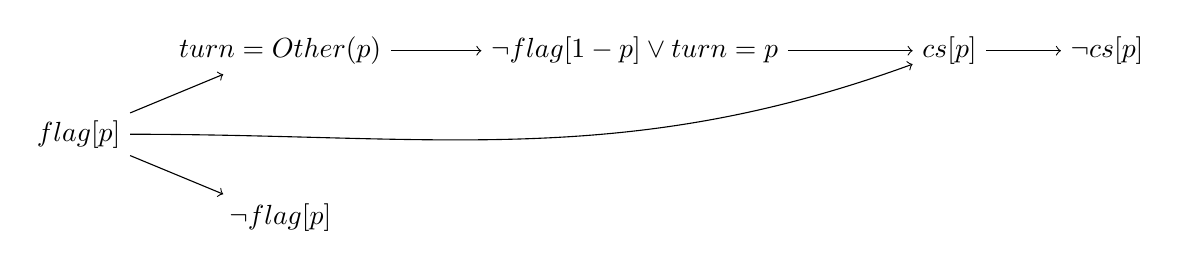
\begin{tikzpicture}[node distance={15mm}, main/.style = {}]
\node[main] (1) {$flag[p]$};
\node[main] (2) [above right of=1,  xshift=15mm] {$turn = Other(p)$};
\node[main] (3) [right of=2,  xshift=30mm] {$\lnot flag[1-p] \vee turn = p$};
\node[main] (4) [right of=3,  xshift=25mm] {$cs[p]$};
\node[main] (5) [right of=4, xshift=5mm] {$\lnot cs[p]$};
\node[main] (6) [below right of=1,  xshift=15mm] {$\lnot flag[p]$};
\draw[->] (1) -- (2);
\draw[->] (2) -- (3);
\draw[->] (3) -- (4);
\draw[->] (4) -- (5);
\draw[->] (1) -- (6);
\draw[->] (1) to [out=0,in=200,looseness=1.0] (4);
\end{tikzpicture}
\end{center}

Because of the safety property $cs[p] => flag[p]$ we can make an aggressive assumption that the user wants us to delay negating $flag[p]$ until after we negate $cs[p]$.  We then produce the following graph:
\begin{center}
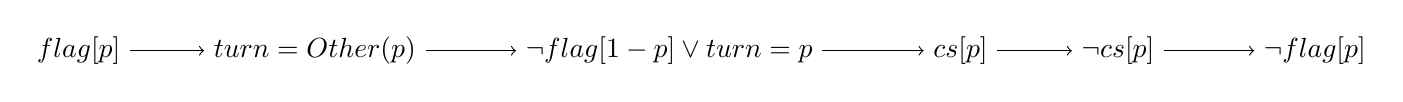
\begin{tikzpicture}[node distance={15mm}, main/.style = {}]
\node[main] (1) {$flag[p]$};
\node[main] (2) [right of=1,  xshift=15mm] {$turn = Other(p)$};
\node[main] (3) [right of=2,  xshift=30mm] {$\lnot flag[1-p] \vee turn = p$};
\node[main] (4) [right of=3,  xshift=22mm] {$cs[p]$};
\node[main] (5) [right of=4, xshift=5mm] {$\lnot cs[p]$};
\node[main] (6) [right of=4,  xshift=30mm] {$\lnot flag[p]$};
\draw[->] (1) -- (2);
\draw[->] (2) -- (3);
\draw[->] (3) -- (4);
\draw[->] (4) -- (5);
\draw[->] (5) -- (6);
\end{tikzpicture}
\end{center}

We now have a pretty good program outline.  We can make a few more aggressive assumption:
\begin{itemize}
	\item Because $flag[p]$ is true and $\lnot flag[p]$ is at the end of the chain we shouldn't consider any instruction that flips $flag[p]$ until we've reached the end of the chain.  
	\item Because $\lnot cs[p]$ is the second to last node of the chain, we shouldn't consider any instruction that turns $cs[p]$ to false before we reach that stage of the chain.  
	\item And so on.  
\end{itemize}

These are aggressive assumptions and they may cause us to miss solutions.  However we attempt to ``take a hint" from the liveness specifications that the user has provided to trim down the search space.  


\subsubsection{Probabilistic Method}
Let $R=$ ``the given program is a prefix to a correct program" and $G=$ ``we see the given liveness graph".  We can use an A* style search, using $P(R|G)$ as our hueristic.  The idea is like \cite{huer} but we will take a slightly different aproach.  Our hueristic for $P(R|G)$ may be very weak and we don't want our search algorithm to get stuck on bad branches so we need to alter A* a bit.  Instead of always choosing to explore the state with the highest probability, instead we explore a random state that's chosen based on the probability of every state in the queue.  We'll need a custom data structure to implement this probabilistic style queue, but for now let's focus on the hueristic.  \\

\textbf{The Hueristic} \\
We can make the problem a bit easier using Baye's formula:
$$P(R|G) \sim P(G|R)P(R)$$

We don't care to include $P(G)$ in our hueristic since this value will be the same for every state.  We can also assign raw probabilities (i.e. our probabilities don't need to sum to 1) due to the nature of our probabilistic queue (see the later section).  Therefore we can let the prior reflect the fact that the longer the program is, the less likely it is to be a prefix to a correct program:
$$P(R)= \frac{1}{1 + \text{number of lines in the program}}$$

As a quick sanity check, an empty (zero line) program has probability 1 of being a prefix to our desired program.  \\

I'll have to think more about $P(G|R)$ \\

A big advantage to calculating $P(G|R)$ is that we take the liveness graph as a big hint by the user.  We will tend to favor programs that run through the whole graph, not just part of it.  Also note that we will increase probabilities by a large (nonlinear) factor because we will be probabilistically choosing a best program over a \textit{very} large number of candidates in the probabilistic queue.  \\

\textbf{Probabilistic Queue} \\
All data is stored in a tree like structure that resembles a heap, except all data is stored at the leaves and associated with a raw probability.  Each node knows the sum of the raw probabilities of all its subtrees.  A consumer wants to choose a random value in the tree, we have the following algorithm starting at the root:
\begin{enumerate}
	\item If the node is a leaf then remove it and return the value.  See the algorithm below for data removal.  
	\item If the node is not a leaf then we choose a subtree to recurse over.  The probability of the left subtree is $\frac{p_L}{p_L + p_R}$, and similar for the right subtree.  Run a Bernoulli trial to determine which subtree to move to.  Repeat the previous step with the root of the chosen subtree.  
\end{enumerate}

This algorithm takes advantage of the chain rule of conditional probability: $P(A,B) = P(B|A)P(A)$.  At each level we make a decision $P(A)$ and then update our probabilities to $P(B|A)$ and proceed down the tree.  Because we calculate the probability of the subchildren as $\frac{p_L}{p_L + p_R}$ (and similar for the right child) we can use raw probabilities (don't sum to 1) which can be far more convenient to work with.  Here's the algorithm for adding a node:
\begin{enumerate}
	\item Add a node with the latest value to the next available slot in the tree.  The parent will be a leaf and needs to be replaced with a node that contains the sum of the raw probabilities of its children.  The old parent now becomes a leaf alongside the newly added data.  
	\item Call a heapify-like routine where bubble up the sum of the raw probabilities
	\item Update the counter to point to the new last node
\end{enumerate}

Removing a value:
\begin{enumerate}
	\item We assume that we already are at the node we wish to remove.  
	\item Swap this value with the last value in the tree.  
	\item The value that was swapped in need to call a heapy-like method to bubble up the new sum of raw probabilities
	\item The value can be removed from the tree.  We need to promote the other child to the slot where the parent was; the data node is still a leaf.  Call heapy-like routine to bubble up the new sum of raw probabilities
	\item Update the counter to point to the new last node
\end{enumerate}

Clearly an array is an appropriate way to implement this data structure since it's similar to a heap in many ways.  Much like a heap, this data structure will use $O(\log{n})$ time for insertion and removal.  It will also use $O(n)$ memory.  


\subsubsection{Discussion}
The probabilistic method has a clear advantage: we don't make assumptions and lose out on the potential to miss solutions.  However it is not clear which method will be better and I will likely choose the method that is easier to implement.  I anticipate that will be the probabilistic method but time will tell.  


\begin{thebibliography}{9}
\bibitem{asdp}
Rajeev Alur, Stavors Tripakis (2017).  ACM SIGACT News, Volume 48, Issue 1.  pp 55–90

\bibitem{mutex}
Wikipedia: Peterson's algorithm.  \url{https://en.wikipedia.org/wiki/Peterson\%27s_algorithm}

\bibitem{il}
Stack Exchange.  \\ \url{https://math.stackexchange.com/questions/77721/number-of-instruction-interleaving}

\bibitem{def}
Alpern, Shneider  \\ \url{https://www.cs.cornell.edu/fbs/publications/DefLiveness.pdf}

\bibitem{huer}
Alur et al. (2018) ACM SIGPLAN Notices, Volume 53, Issue 4  \\ \url{https://dl.acm.org/doi/pdf/10.1145/3296979.3192410}
\end{thebibliography}

\end{document}













